\documentclass[conference]{IEEEtran}

\usepackage[pdftex]{graphicx}
\graphicspath{{./}}
\DeclareGraphicsExtensions{.pdf,.jpeg,.png}

\usepackage[cmex10]{amsmath}
\usepackage{amssymb}
\usepackage{mathabx}
\usepackage{algorithmic}
\usepackage{array}
\usepackage{mdwmath}
\usepackage{mdwtab}
\usepackage{eqparbox}
\usepackage{url}
\usepackage{booktabs}
\usepackage{multirow}
\hyphenation{op-tical net-works semi-conduc-tor}

\begin{document}

\title{\LARGE Implementación y Entrenamiento desde Cero de una Red Neuronal Convolucional en CUDA/C++ para la Clasificación de Dígitos MNIST}

\author{
  \IEEEauthorblockN{Diego Alonso Zanabria Sacsi\IEEEauthorrefmark{1}, \\
  Sergio Ahmed Castillo Sancho\IEEEauthorrefmark{1}}
  \IEEEauthorblockA{\IEEEauthorrefmark{1}\textit{Escuela de Ciencia de la Computación} \\
  \textit{Universidad Nacional de San Agustín} \\
  Arequipa, Perú \\
  \{dzanabria, scastillos\}@unsa.edu.pe}
  \and
  \IEEEauthorblockN{Diego Francisco Apaza Andaluz\IEEEauthorrefmark{1}, \\
  Owen Haziel Roque Sosa\IEEEauthorrefmark{1}}
  \IEEEauthorblockA{\IEEEauthorrefmark{1}\textit{Escuela de Ciencia de la Computación} \\
  \textit{Universidad Nacional de San Agustín} \\
  Arequipa, Perú \\
  \{dapazaan, oroque\}@unsa.edu.pe}
}

\maketitle

\begin{abstract}
Las redes neuronales convolucionales (CNN) siguen siendo, más de veinticinco años después de su formulación original, la arquitectura de referencia para tareas de clasificación de imágenes de baja y mediana complejidad, gracias al sesgo inductivo que introduce la operación de convolución: localidad, compartición de pesos e invarianza aproximada a la traslación. En este trabajo se implementa desde cero, en C++ y CUDA, una CNN compacta (206{,}922 parámetros) para la clasificación de dígitos manuscritos del conjunto de datos MNIST, sin recurrir a bibliotecas de álgebra lineal o de aprendizaje profundo de alto nivel. Se describe el marco teórico de la convolución 2D, la reducción por máximos (\emph{max-pooling}) y su implementación eficiente mediante la técnica \emph{im2col} combinada con una multiplicación de matrices (GEMM) genérica en CUDA, así como los detalles de optimización mediante AdamW con una política de \emph{warmup} lineal y decaimiento cosenoidal de la tasa de aprendizaje. El modelo fue entrenado durante 20 épocas sobre una GPU NVIDIA GeForce RTX 4060 Laptop, alcanzando una exactitud de prueba final de 99.26\% (máxima de 99.28\% en la época 18) y una pérdida de entropía cruzada de 0.0260 sobre las 10{,}000 imágenes del conjunto de prueba. Se presentan y discuten las curvas de entrenamiento, la matriz de confusión, los filtros aprendidos por la primera capa convolucional y sus mapas de activación, concluyendo que el sesgo inductivo convolucional permite una convergencia más rápida y una exactitud ligeramente superior a la de un Vision Transformer de tamaño comparable entrenado bajo condiciones equivalentes sobre el mismo conjunto de datos.
\end{abstract}

\IEEEoverridecommandlockouts
\begin{IEEEkeywords}
Redes neuronales convolucionales, CNN, MNIST, aprendizaje profundo, CUDA, im2col, AdamW, clasificación de imágenes.
\end{IEEEkeywords}

\IEEEpeerreviewmaketitle


% ===================
% # I. Introducción #
% ===================
\section{Introducción}

Las redes neuronales convolucionales (\emph{Convolutional Neural Networks}, CNN) fueron introducidas en su forma moderna por LeCun et al. \cite{lecun1998mnist} con la arquitectura LeNet-5, aplicada precisamente al reconocimiento de dígitos manuscritos. A diferencia de un perceptrón multicapa totalmente conectado, una CNN explota la estructura espacial local de las imágenes mediante filtros convolucionales que se aplican de forma deslizante y comparten sus parámetros a lo largo de toda la entrada, lo que reduce drásticamente el número de parámetros entrenables respecto de una capa densa equivalente y otorga al modelo un sesgo inductivo de localidad e invarianza aproximada a la traslación. Este principio, combinado con la reducción progresiva de la resolución espacial mediante \emph{pooling}, permitió a arquitecturas como AlexNet \cite{krizhevsky2012imagenet} popularizar las CNN como el estándar de facto para la clasificación de imágenes durante la década siguiente, hasta la reciente irrupción de los Vision Transformers \cite{dosovitskiy2020image}, que prescinden por completo de la convolución.

El problema abordado en este trabajo es doble. Primero, un problema de \emph{implementación}: construir, sin depender de frameworks de alto nivel como PyTorch o TensorFlow ni de bibliotecas optimizadas como cuDNN o cuBLAS, una CNN funcional en C++/CUDA, implementando manualmente cada operación (convolución 2D vía \emph{im2col} y GEMM, \emph{max-pooling}, activación ReLU, capas totalmente conectadas, \emph{dropout}, retropropagación y el optimizador AdamW) como kernels de GPU. Segundo, un problema de \emph{aprendizaje automático}: validar que dicha implementación converge correctamente y logra un desempeño competitivo en la tarea de clasificación de dígitos manuscritos MNIST \cite{lecun1998mnist}, banco de pruebas estándar para verificar la corrección de nuevas arquitecturas e implementaciones.

La motivación de implementar el modelo "desde cero" es la misma que en trabajos previos de este grupo sobre arquitecturas basadas en atención \cite{dosovitskiy2020image}: el control total sobre cada operación matemática involucrada permite verificar la corrección numérica de la implementación y medir de forma directa el impacto de decisiones de diseño (número de filtros, profundidad, tasa de \emph{dropout}) sobre el rendimiento final y el consumo de memoria de la GPU. Adicionalmente, al compartir el mismo conjunto de datos, tamaño de lote y metodología de entrenamiento (AdamW con \emph{warmup} y decaimiento cosenoidal) que un trabajo companion sobre un Vision Transformer entrenado en las mismas condiciones, este trabajo permite una comparación directa y controlada entre un modelo con sesgo inductivo convolucional y uno sin él, sobre una misma tarea.

El resto del artículo se organiza de la siguiente manera: la Sección II presenta el marco teórico de la convolución 2D, el \emph{max-pooling} y los componentes de optimización; la Sección III describe la metodología de implementación y la configuración experimental; la Sección IV presenta y discute los resultados obtenidos; finalmente, la Sección V expone las conclusiones y el trabajo futuro.


% ==========================
% # II. Marco Teórico #
% ==========================
\section{Marco Teórico}

\subsection{Convolución 2D}
Dada una entrada $X \in \mathbb{R}^{C_{in} \times H \times W}$ con $C_{in}$ canales, una capa convolucional aplica un banco de $C_{out}$ filtros $W_k \in \mathbb{R}^{C_{in}\times K_H\times K_W}$, produciendo una salida $Y \in \mathbb{R}^{C_{out}\times H'\times W'}$ cuyo elemento en la posición $(k, i, j)$ se calcula como:
\begin{equation}
Y_{k,i,j} = b_k + \sum_{c=1}^{C_{in}}\sum_{u=0}^{K_H-1}\sum_{v=0}^{K_W-1} W_{k,c,u,v} \, X_{c,\, i\cdot s + u - p,\, j\cdot s + v - p}
\end{equation}
donde $s$ es el desplazamiento (\emph{stride}), $p$ el relleno (\emph{padding}) y $b_k$ el sesgo del filtro $k$. A diferencia de una capa totalmente conectada, los pesos $W_k$ se comparten para todas las posiciones espaciales $(i,j)$, lo que reduce el número de parámetros de $O(C_{in}\cdot C_{out}\cdot H\cdot W)$ a $O(C_{in}\cdot C_{out}\cdot K_H\cdot K_W)$ y confiere a la capa una invarianza aproximada a la traslación.

\subsection{Implementación eficiente vía im2col + GEMM}
Calcular la ecuación (1) mediante bucles anidados explícitos resulta ineficiente en una GPU. Siguiendo la práctica estándar en la implementación de motores de aprendizaje profundo, la convolución se reformula como una única multiplicación de matrices (GEMM). La transformación \emph{im2col} reorganiza cada ventana receptiva de la entrada en una columna de una matriz $\mathrm{Col}\in\mathbb{R}^{(C_{in}K_HK_W)\times(N\cdot H'W')}$, de modo que la convolución completa del lote se obtiene como:
\begin{equation}
Y_{[C_{out}\times NH'W']} = W_{[C_{out}\times C_{in}K_HK_W]} \cdot \mathrm{Col}_{[C_{in}K_HK_W \times NH'W']}
\end{equation}
seguida de la suma del sesgo por fila. El gradiente respecto de la entrada se obtiene de forma simétrica: $\mathrm{dCol} = W^T \cdot \mathrm{d}Y$, seguido de la operación inversa \emph{col2im}, que acumula (mediante sumas atómicas) las contribuciones de las ventanas solapadas sobre el tensor de entrada. Los gradientes de los pesos y del sesgo se calculan como $\mathrm{d}W = \mathrm{d}Y\cdot\mathrm{Col}^T$ y $\mathrm{d}b_k=\sum_{n,i,j}\mathrm{d}Y_{k,n,i,j}$, respectivamente. Esta formulación permite reutilizar un único kernel de GEMM tileado en memoria compartida como primitiva de cómputo tanto para las capas convolucionales como para las capas totalmente conectadas, de manera análoga a como el GEMM genérico constituye el primitivo central en la implementación de un Transformer \cite{vaswani2017attention}.

\subsection{Activación ReLU}
Se emplea la unidad lineal rectificada (ReLU) \cite{nair2010rectified} como no linealidad tras cada capa convolucional y tras la primera capa totalmente conectada:
\begin{equation}
\mathrm{ReLU}(x) = \max(0, x)
\end{equation}
Su gradiente es la función indicadora $\mathbb{1}[x>0]$, lo que evita el problema de desvanecimiento del gradiente característico de las activaciones saturantes (sigmoide, tangente hiperbólica) y tiene un costo computacional mínimo.

\subsection{Max-pooling}
La capa de \emph{max-pooling} reduce la resolución espacial de los mapas de activación tomando el valor máximo dentro de ventanas disjuntas de tamaño $2\times2$:
\begin{equation}
Y_{c,i,j} = \max_{0\le u,v <2} X_{c,\,2i+u,\,2j+v}
\end{equation}
Esta operación introduce invarianza local a pequeñas traslaciones y reduce a la cuarta parte el número de activaciones que deben propagarse a la siguiente capa, disminuyendo tanto el costo computacional como el número de parámetros de las capas totalmente conectadas subsiguientes. En la retropropagación, el gradiente de cada ventana de salida se enruta únicamente hacia la posición que produjo el máximo (registrada durante el paso hacia adelante), y es cero en el resto de posiciones de la ventana.

\subsection{Dropout}
Para mitigar el sobreajuste en la capa totalmente conectada de mayor tamaño, se aplica \emph{dropout} \cite{srivastava2014dropout} con probabilidad $p=0.25$ tras la primera capa densa: durante el entrenamiento, cada activación se anula de forma independiente con probabilidad $p$ y las activaciones restantes se reescalan por $1/(1-p)$ para mantener el valor esperado; durante la inferencia, la capa se comporta como la identidad.

\subsection{Arquitectura de la CNN}
El modelo implementado sigue el patrón clásico de LeNet \cite{lecun1998mnist} con dos bloques convolucionales seguidos de un clasificador totalmente conectado:
\begin{align}
\nonumber X_0 \in \mathbb{R}^{1\times28\times28} \xrightarrow{\text{Conv }3\times3,\,16} &\;\mathrm{ReLU} \xrightarrow{\text{Pool }2\times2} X_1 \in \mathbb{R}^{16\times14\times14} \\
\nonumber X_1 \xrightarrow{\text{Conv }3\times3,\,32} &\;\mathrm{ReLU} \xrightarrow{\text{Pool }2\times2} X_2 \in \mathbb{R}^{32\times7\times7} \\
\nonumber \mathrm{vec}(X_2)\in\mathbb{R}^{1568} \xrightarrow{\text{FC}} &\;128 \xrightarrow{\mathrm{ReLU},\,\mathrm{Dropout}} \xrightarrow{\text{FC}} 10
\end{align}
Ambas capas convolucionales usan relleno $p=1$ y desplazamiento $s=1$, preservando la resolución espacial antes de cada reducción por \emph{pooling}. El resultado final de 10 unidades corresponde a los logits de las 10 clases de dígitos (0-9).

\subsection{Cabeza de clasificación}
Los logits se normalizan mediante una función softmax para obtener una distribución de probabilidad sobre las 10 clases, entrenada mediante la pérdida de entropía cruzada:
\begin{equation}
\mathcal{L} = -\sum_{c=1}^{10} y_c \log(\hat{y}_c)
\end{equation}
El gradiente combinado de softmax y entropía cruzada respecto de los logits adopta la forma compacta $\partial\mathcal{L}/\partial z_c = \hat{y}_c - y_c$, que se calcula en un único kernel fusionado para evitar la propagación de errores de redondeo a través de dos pasos separados.

\subsection{Optimización: AdamW}
El entrenamiento se realiza con el optimizador AdamW \cite{loshchilov2017decoupled}, que desacopla la regularización por decaimiento de pesos de la actualización basada en el gradiente:
\begin{align}
m_t &= \beta_1 m_{t-1} + (1-\beta_1)g_t \\
v_t &= \beta_2 v_{t-1} + (1-\beta_2)g_t^2 \\
\theta_t &= \theta_{t-1} - \eta\left(\frac{\hat{m}_t}{\sqrt{\hat{v}_t}+\epsilon} + \lambda\theta_{t-1}\right)
\end{align}
donde $\hat{m}_t$ y $\hat{v}_t$ son los estimadores corregidos por sesgo de los momentos de primer y segundo orden, $\eta$ la tasa de aprendizaje y $\lambda$ el coeficiente de decaimiento de pesos.

\subsection{Programación de la tasa de aprendizaje}
Se emplea la misma política de \emph{warmup} lineal seguido de decaimiento cosenoidal utilizada en trabajos previos de este grupo con arquitecturas basadas en atención, dado que estabiliza el entrenamiento en las primeras iteraciones y favorece la convergencia fina hacia el final:
\begin{equation}
\eta(t) =
\begin{cases}
\eta_{\max}\dfrac{t}{t_{\mathrm{w}}} & t \le t_{\mathrm{w}} \\[8pt]
\eta_{\min} + \dfrac{\eta_{\max}-\eta_{\min}}{2}\left(1+\cos\left(\pi\dfrac{t-t_{\mathrm{w}}}{T-t_{\mathrm{w}}}\right)\right) & t > t_{\mathrm{w}}
\end{cases}
\end{equation}
donde $T$ es el número total de pasos de entrenamiento y $t_{\mathrm{w}}$ el número de pasos de \emph{warmup}. Esta política se ilustra en la Figura~\ref{fig:training} (panel derecho).

\begin{figure*}[htpb]
\centering
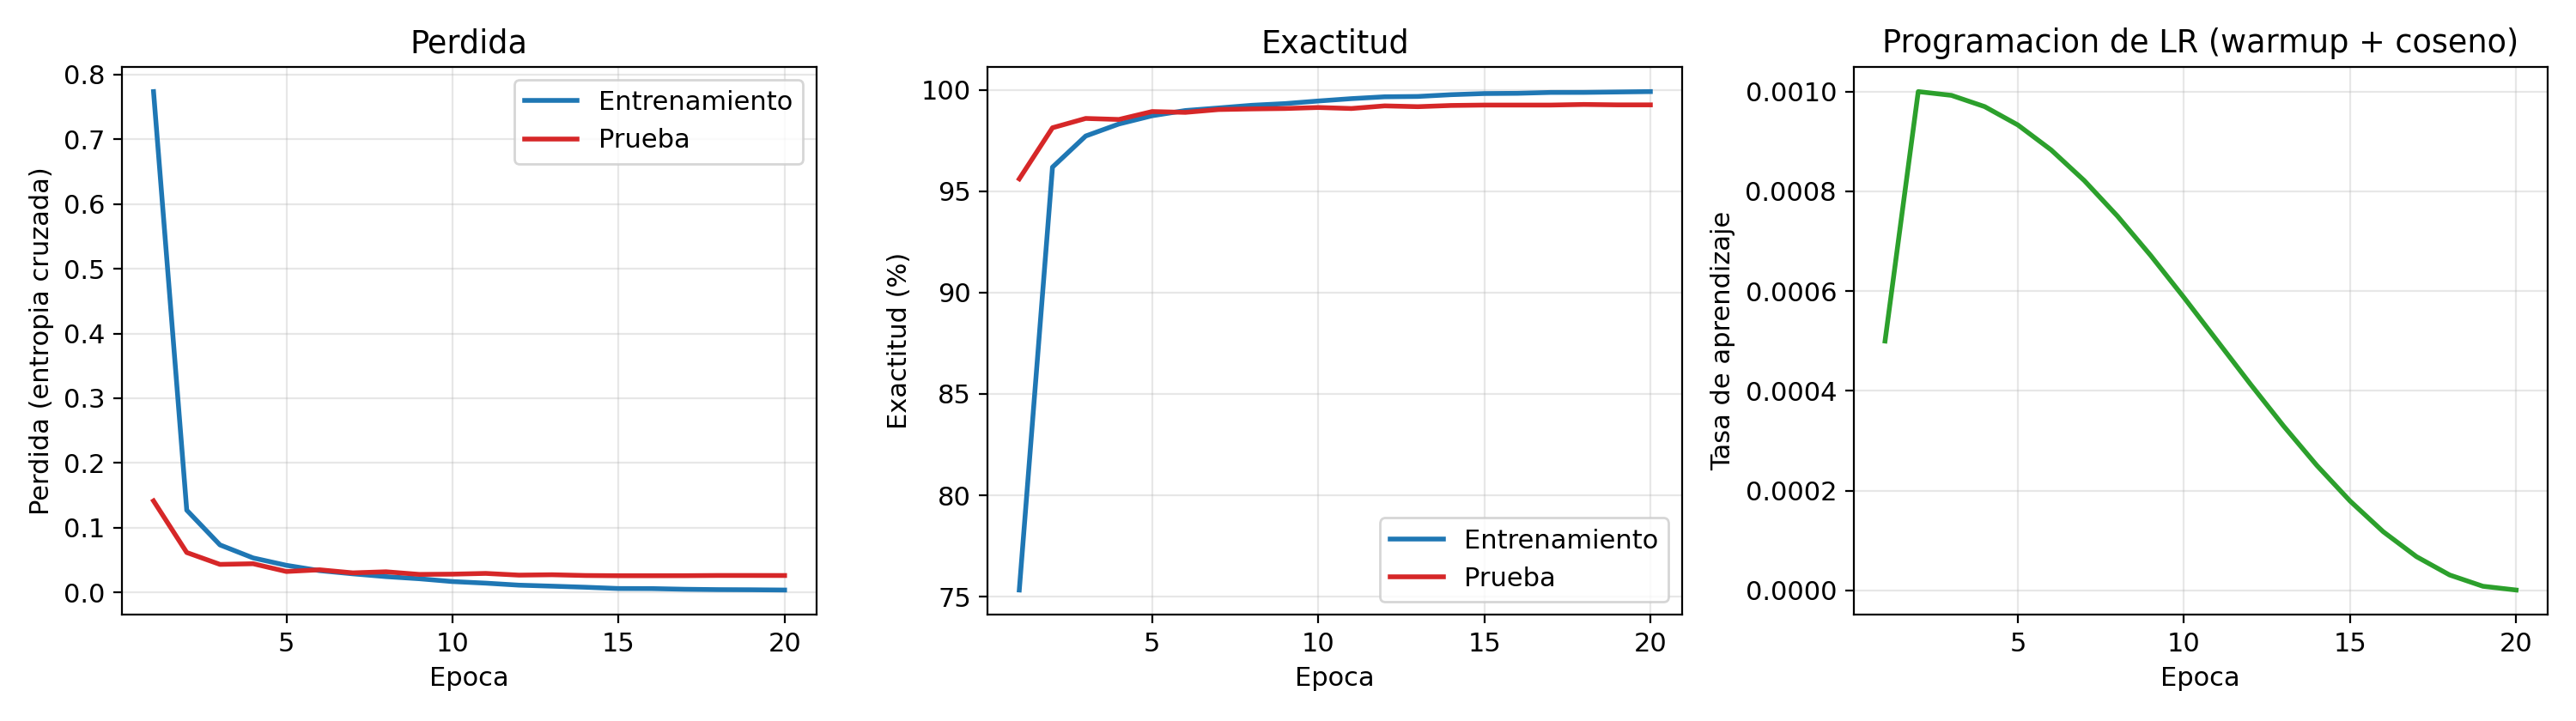
\includegraphics[width=1\linewidth]{cnn_training.png}
\caption{Curvas de entrenamiento de la CNN sobre MNIST: (izquierda) pérdida de entropía cruzada, (centro) exactitud, (derecha) programación de la tasa de aprendizaje (\emph{warmup} + decaimiento cosenoidal).}
\label{fig:training}
\end{figure*}

% ================================
% # III. Metodología #
% ================================
\section{Metodología e Implementación}

\subsection{Arquitectura de software}
El sistema fue implementado en C++17 con núcleos CUDA personalizados para todas las operaciones computacionalmente intensivas: una multiplicación de matrices genérica (GEMM) tileada en memoria compartida con soporte de transposición lógica de operandos, las transformaciones \emph{im2col}/\emph{col2im} para la convolución, \emph{max-pooling} con registro de índices de máximo, activación ReLU, \emph{dropout} (con máscaras generadas mediante la API de host de cuRAND), softmax fusionado con entropía cruzada, y el optimizador AdamW. Las capas de más alto nivel (\texttt{Conv2D}, \texttt{MaxPool2D}, \texttt{Linear}, \texttt{Dropout}) se organizan como clases en C++ que orquestan las llamadas a los kernels CUDA subyacentes y reservan sus propios búferes intermedios (columnas \emph{im2col}, índices de máximo) para un tamaño de lote máximo, admitiendo tamaños de lote variables (\mbox{$n\le$ lote máximo}) para poder evaluar el conjunto de prueba completo sin descartar el lote final incompleto. La construcción del proyecto se gestiona mediante CMake, enlazando contra el \emph{CUDA Toolkit} (v13.3) y la biblioteca cuRAND.

\subsection{Conjunto de datos}
Se utilizó el conjunto de datos MNIST \cite{lecun1998mnist}, compuesto por 60{,}000 imágenes de entrenamiento y 10{,}000 imágenes de prueba de dígitos manuscritos en escala de grises de $28\times28$ píxeles, distribuidos en 10 clases balanceadas (dígitos 0 a 9), normalizadas al rango $[0,1]$.

\subsection{Configuración del modelo}
La Tabla~\ref{tab:hyperparams} resume la arquitectura y los hiperparámetros empleados. Los pesos de todas las capas se inicializaron con la estrategia de He (Kaiming) \cite{he2015delving}, adecuada para activaciones ReLU, y los sesgos se inicializaron en cero.

\begin{table}[h]
\centering
\caption{Configuración de la CNN e hiperparámetros de entrenamiento}
\label{tab:hyperparams}
\begin{tabular}{ll}
\toprule
\textbf{Parámetro} & \textbf{Valor} \\
\midrule
Tamaño de imagen & $28\times28$ \\
Conv1 & $16$ filtros $3\times3$, pad 1 \\
Conv2 & $32$ filtros $3\times3$, pad 1 \\
Pooling & Max $2\times2$ (ambos bloques) \\
Dimensión aplanada & $32\times7\times7=1568$ \\
Capa oculta FC & 128 \\
Dropout & 0.25 \\
Parámetros totales & 206{,}922 \\
\midrule
Optimizador & AdamW ($\beta_1=0.9$, $\beta_2=0.999$) \\
Decaimiento de pesos & $10^{-4}$ \\
Tamaño de lote & 128 \\
Épocas & 20 \\
Lotes por época & 469 \\
Pasos totales / warmup & 9{,}380 / 938 (10\%) \\
Tasa de aprendizaje máx./mín. & $10^{-3}$ / $10^{-6}$ \\
Política de LR & Warmup lineal + coseno \\
\bottomrule
\end{tabular}
\end{table}

\subsection{Hardware}
El entrenamiento se ejecutó sobre una GPU NVIDIA GeForce RTX 4060 Laptop (arquitectura Ada Lovelace, \emph{compute capability} 8.9, 24 \emph{streaming multiprocessors}, 8{,}188 MiB de memoria disponible), con CUDA 13.3, controlador 592.82. El consumo de memoria de la GPU tras inicializar el modelo y sus búferes de activación fue de aproximadamente 1{,}167.5 MiB, muy por debajo de la capacidad total de la tarjeta.

\subsection{Protocolo experimental}
El modelo se entrenó durante 20 épocas, evaluando la pérdida y exactitud tanto en el conjunto de entrenamiento como en el de prueba al finalizar cada época. Al concluir el entrenamiento se calculó la matriz de confusión sobre el conjunto de prueba completo (10{,}000 muestras), se exportaron los 16 filtros de la primera capa convolucional, los mapas de activación de conv1 y conv2 para una imagen de muestra, y una muestra cualitativa de 24 predicciones sobre el conjunto de prueba.


% ==========================
% # IV. Resultados #
% ==========================
\section{Resultados}

\subsection{Curvas de entrenamiento}
La Figura~\ref{fig:training} muestra la evolución de la pérdida de entropía cruzada, la exactitud y la programación de la tasa de aprendizaje a lo largo de las 20 épocas de entrenamiento.

La convergencia es notablemente rápida: la exactitud de prueba alcanza 95.61\% al finalizar la primera época y supera el 98\% en la segunda. A partir de la quinta época, la exactitud de prueba se estabiliza por encima de 98.9\%, mientras que la exactitud de entrenamiento continúa aumentando hasta 99.92\% en la época final, lo que evidencia un ligero sobreajuste hacia el final del entrenamiento —esperable dado el aumento sostenido de la capacidad efectiva del modelo a medida que la tasa de aprendizaje decae— sin que ello perjudique la exactitud de prueba, que permanece estable en torno a 99.2-99.3\% durante las últimas diez épocas. La mejor exactitud de prueba alcanzada fue de 99.28\%, obtenida en la época 18, mientras que el resultado final tras las 20 épocas fue de 99.26\%, con una pérdida de prueba de 0.0260. El panel de la tasa de aprendizaje evidencia la fase de \emph{warmup} durante los primeros pasos, alcanzando el valor pico de $10^{-3}$ antes de la segunda época, seguida del decaimiento cosenoidal suave hasta $10^{-6}$ al final del entrenamiento. El tiempo de cómputo por época, dominado por las 469 iteraciones de entrenamiento y las 79 de evaluación, fue de entre 3.2 y 7.6 segundos, con una media aproximada de 5.8 segundos, sobre una GPU compartida con otros procesos del sistema en el momento de la ejecución.

\subsection{Matriz de confusión}
La Figura~\ref{fig:confusion} presenta la matriz de confusión calculada sobre el conjunto de prueba completo (10{,}000 muestras).

\begin{figure}[ht!]
\centering
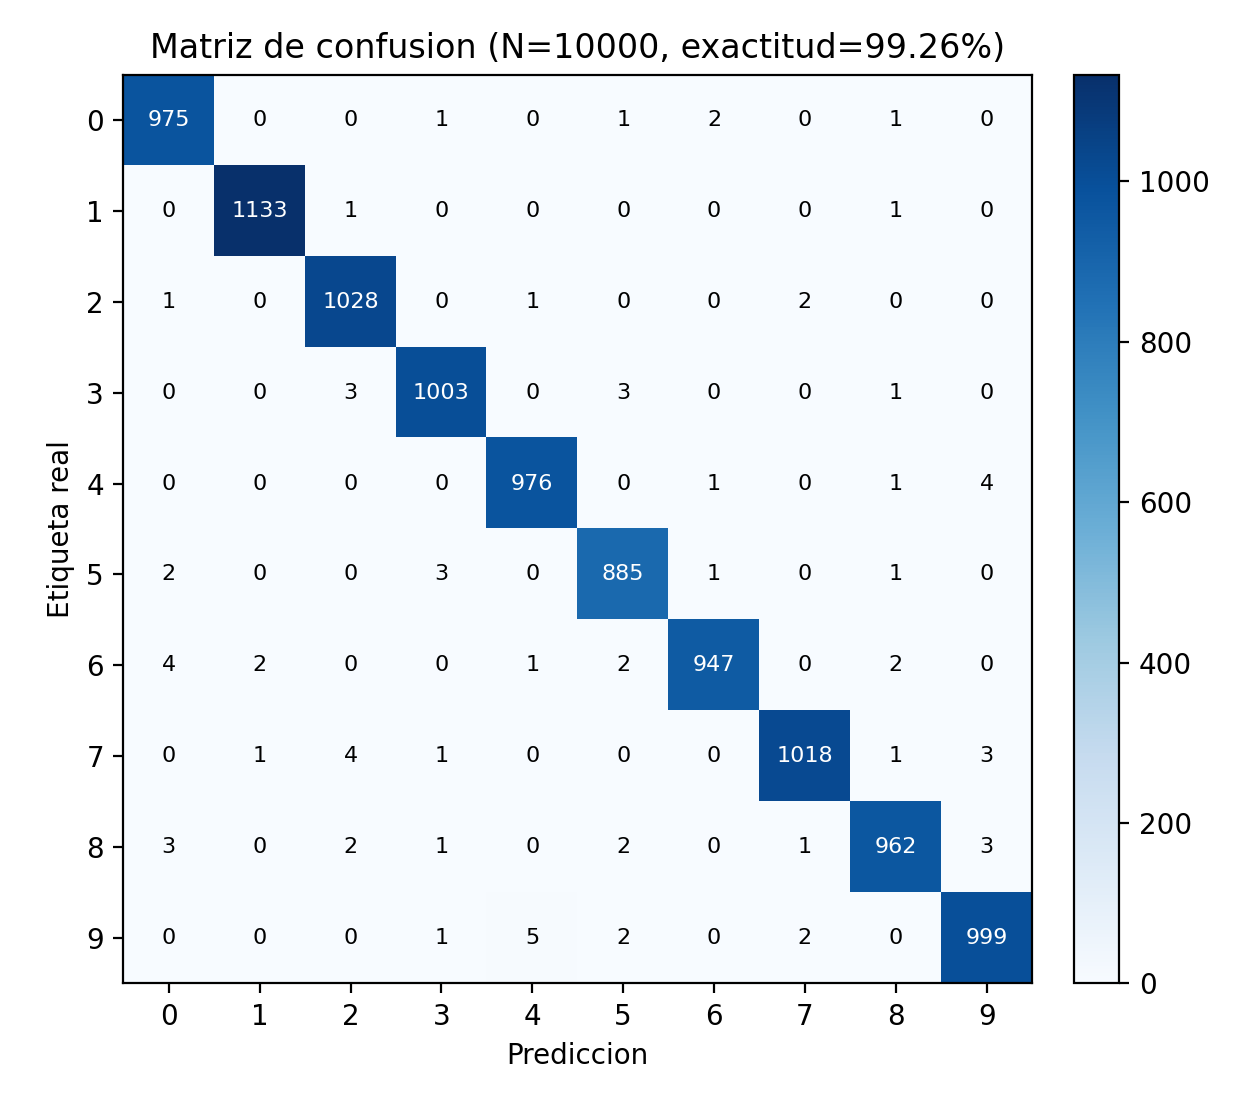
\includegraphics[width=3.2in]{cnn_confusion.png}
\caption{Matriz de confusión de la CNN sobre el conjunto de prueba de MNIST (10{,}000 muestras).}
\label{fig:confusion}
\end{figure}

La matriz evidencia una diagonal fuertemente dominante, consistente con la exactitud global de 99.26\%. Las confusiones más frecuentes son 9$\to$4 (5 casos), y con 4 casos cada una: 7$\to$2, 6$\to$0 y 4$\to$9. Estas confusiones son, nuevamente, explicables desde el punto de vista morfológico: los pares 4/9 y 6/0 comparten trazos curvos que pueden volverse ambiguos en caligrafías con lazos poco cerrados o astas cortas, mientras que 7/2 comparte el trazo diagonal descendente cuando el 7 se escribe sin la barra horizontal media. En comparación con un Vision Transformer de tamaño comparable entrenado bajo el mismo protocolo sobre el mismo conjunto de datos \cite{dosovitskiy2020image}, la CNN aquí presentada exhibe un patrón de errores cualitativamente similar (predominan las confusiones 4/9, 7/2 y 5/3), pero con una magnitud absoluta menor en casi todas las clases, lo que es coherente con la exactitud global superior obtenida (99.26\% frente a 98.68\%).

\subsection{Filtros aprendidos}
La Figura~\ref{fig:filters} muestra los 16 filtros $3\times3$ aprendidos por la primera capa convolucional.

\begin{figure}[ht!]
\centering
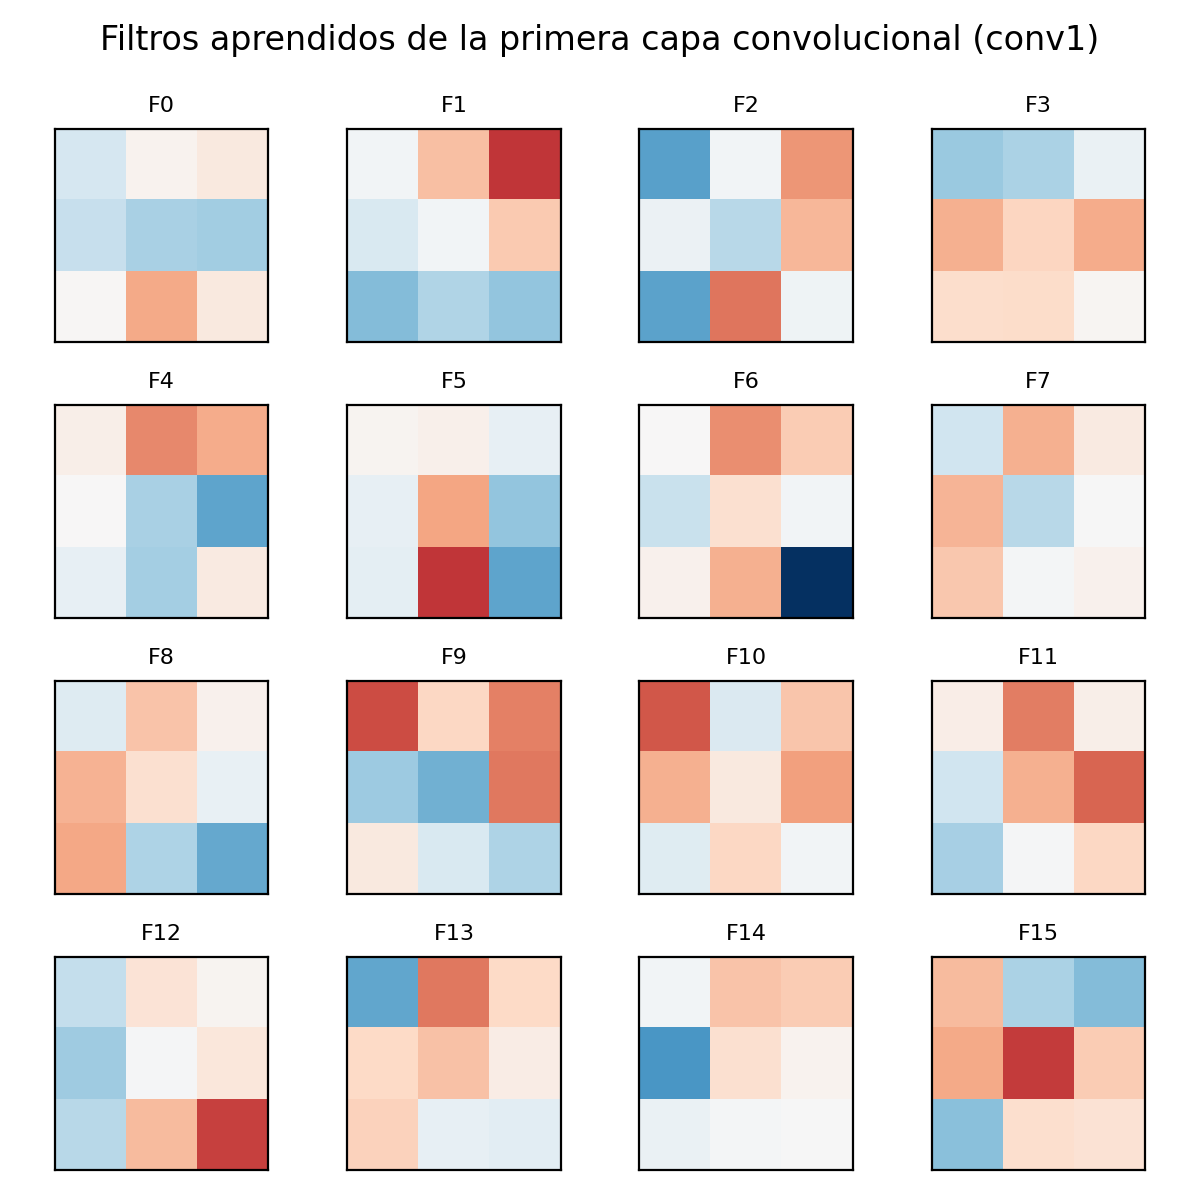
\includegraphics[width=3.2in]{cnn_filters.png}
\caption{Filtros de $3\times3$ aprendidos por la capa conv1 (16 canales de salida sobre 1 canal de entrada).}
\label{fig:filters}
\end{figure}

A diferencia de los mapas de atención de un Transformer, en una CNN los propios pesos de la primera capa son directamente interpretables como detectores de bordes y gradientes de intensidad locales. Se observa que la mayoría de los filtros (por ejemplo F1, F6, F9, F11) desarrollaron patrones de tipo detector de borde orientado, con signos opuestos concentrados en lados contiguos del núcleo $3\times3$, mientras que otros (F0, F14) se asemejan a detectores de borde horizontal o vertical más simples. Ningún filtro colapsó a una configuración degenerada (constante o de ruido), lo que sugiere que las 16 unidades de la primera capa se especializaron en direcciones de gradiente complementarias durante el entrenamiento.

\subsection{Mapas de activación}
La Figura~\ref{fig:featuremaps} muestra los mapas de activación producidos por conv1 (16 canales, $28\times28$) y conv2 (32 canales, $14\times14$) para una imagen de prueba del dígito 9, correctamente clasificada.

\begin{figure}[ht!]
\centering
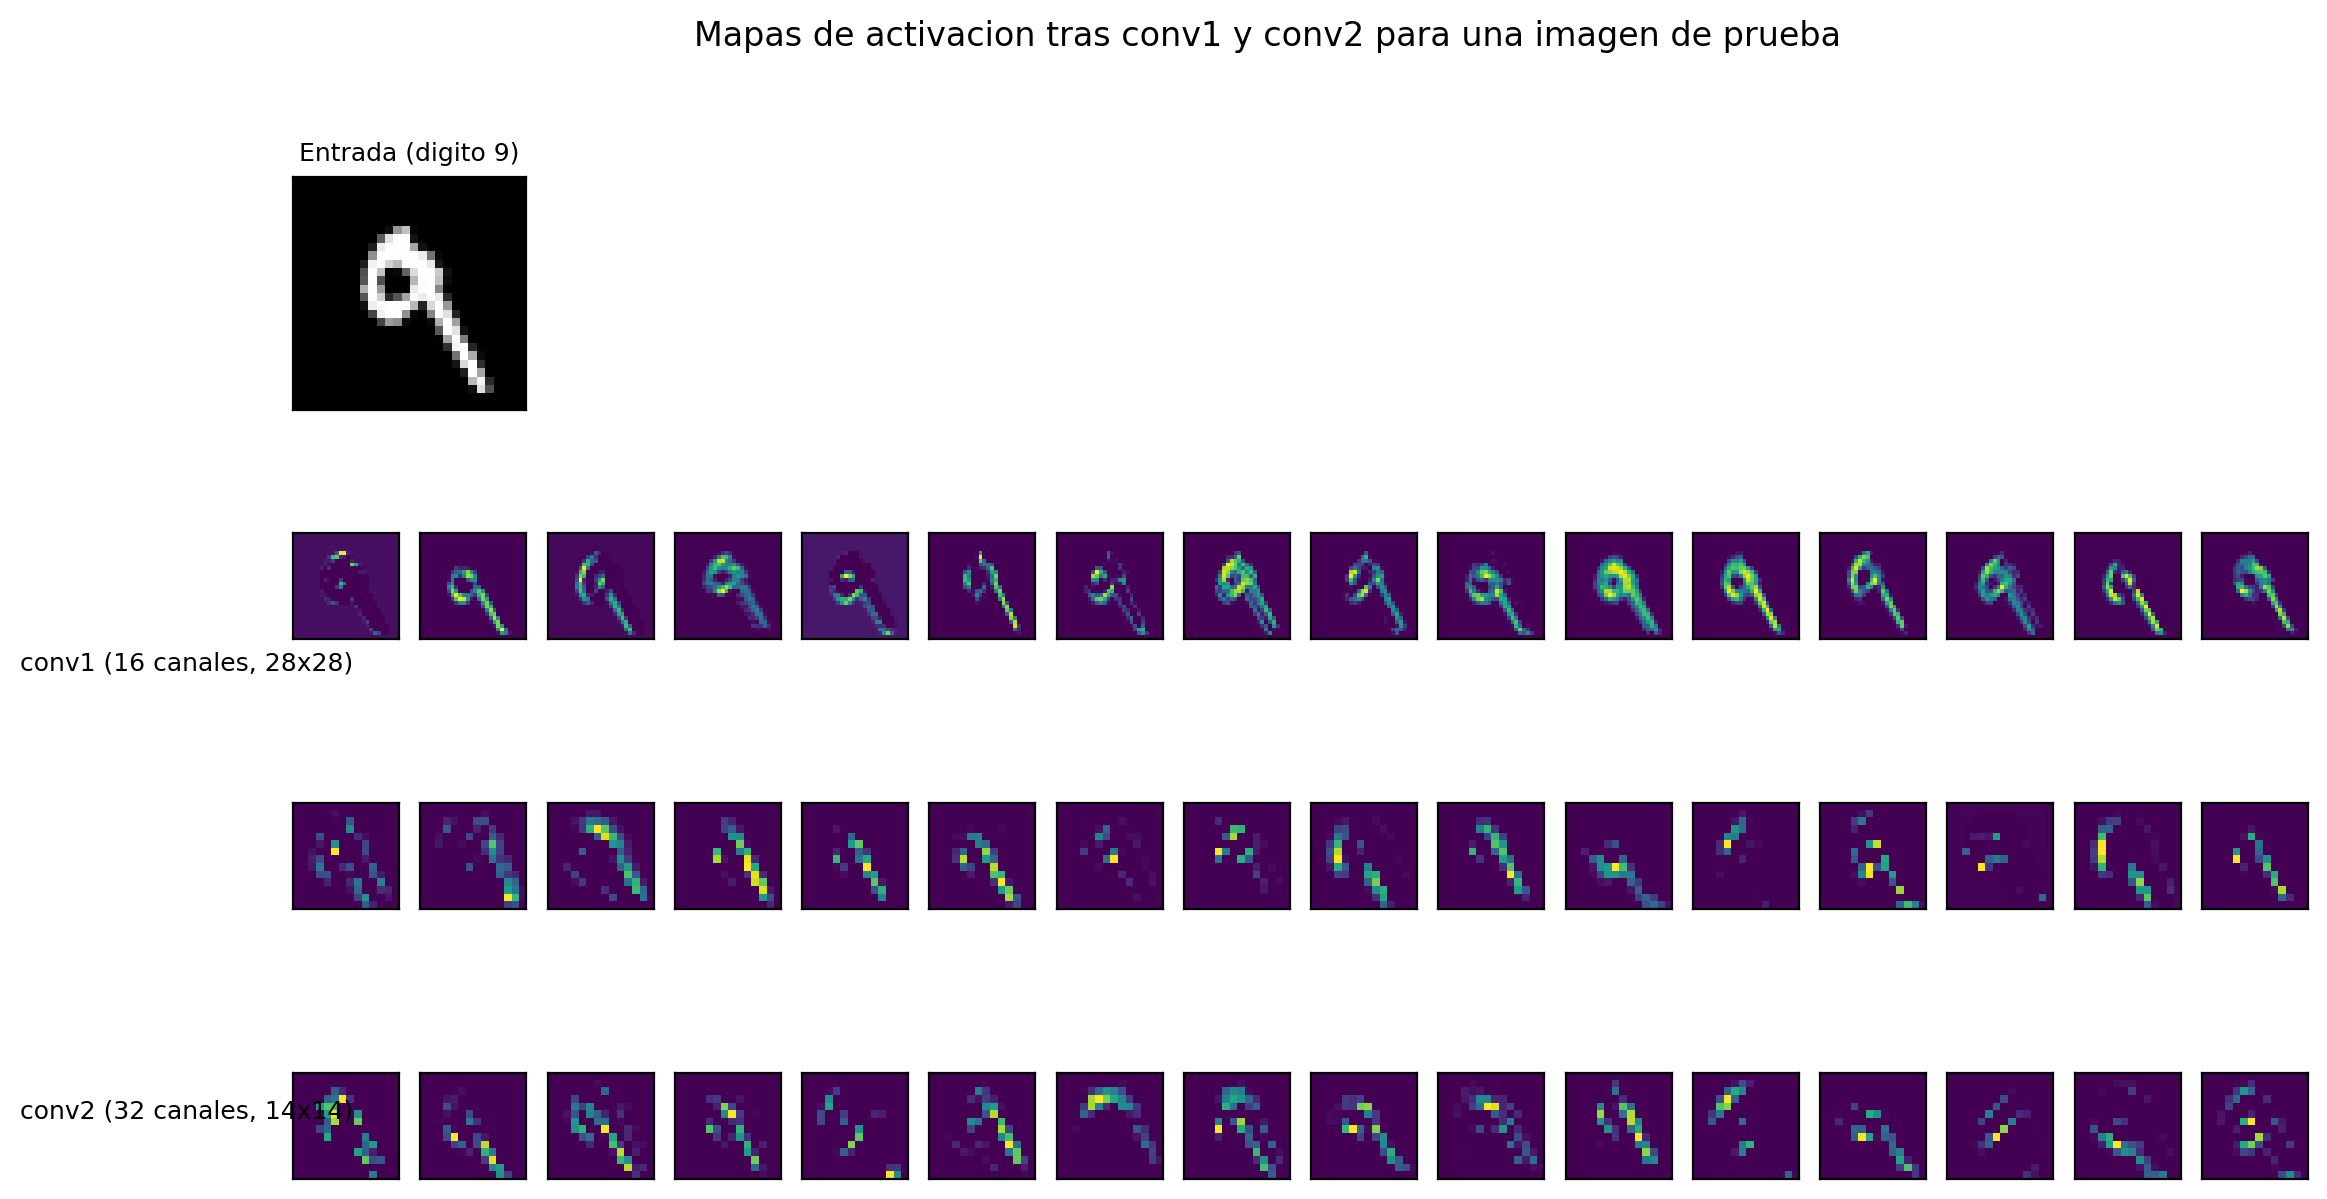
\includegraphics[width=3.5in]{cnn_featuremaps.png}
\caption{Mapas de activación de conv1 y conv2 (tras ReLU) para una imagen de prueba.}
\label{fig:featuremaps}
\end{figure}

Los canales de conv1 muestran respuestas nítidamente localizadas sobre el trazo del dígito, con distintos canales resaltando selectivamente el lazo superior, el asta diagonal, o los bordes de ambos rasgos simultáneamente —comportamiento consistente con los filtros de tipo detector de bordes observados en la Figura~\ref{fig:filters}. Tras el segundo bloque convolucional, los mapas de conv2 muestran activaciones más dispersas y de mayor nivel de abstracción, con varios canales respondiendo a la combinación completa lazo-asta característica del dígito 9 más que a bordes locales aislados, lo que evidencia la composicionalidad jerárquica típica de las CNN: cada capa convolucional adicional integra información de una vecindad espacial mayor de la capa anterior.

\subsection{Predicciones cualitativas}
La Figura~\ref{fig:predictions} muestra 24 ejemplos de predicciones sobre el conjunto de prueba.

\begin{figure}[ht!]
\centering
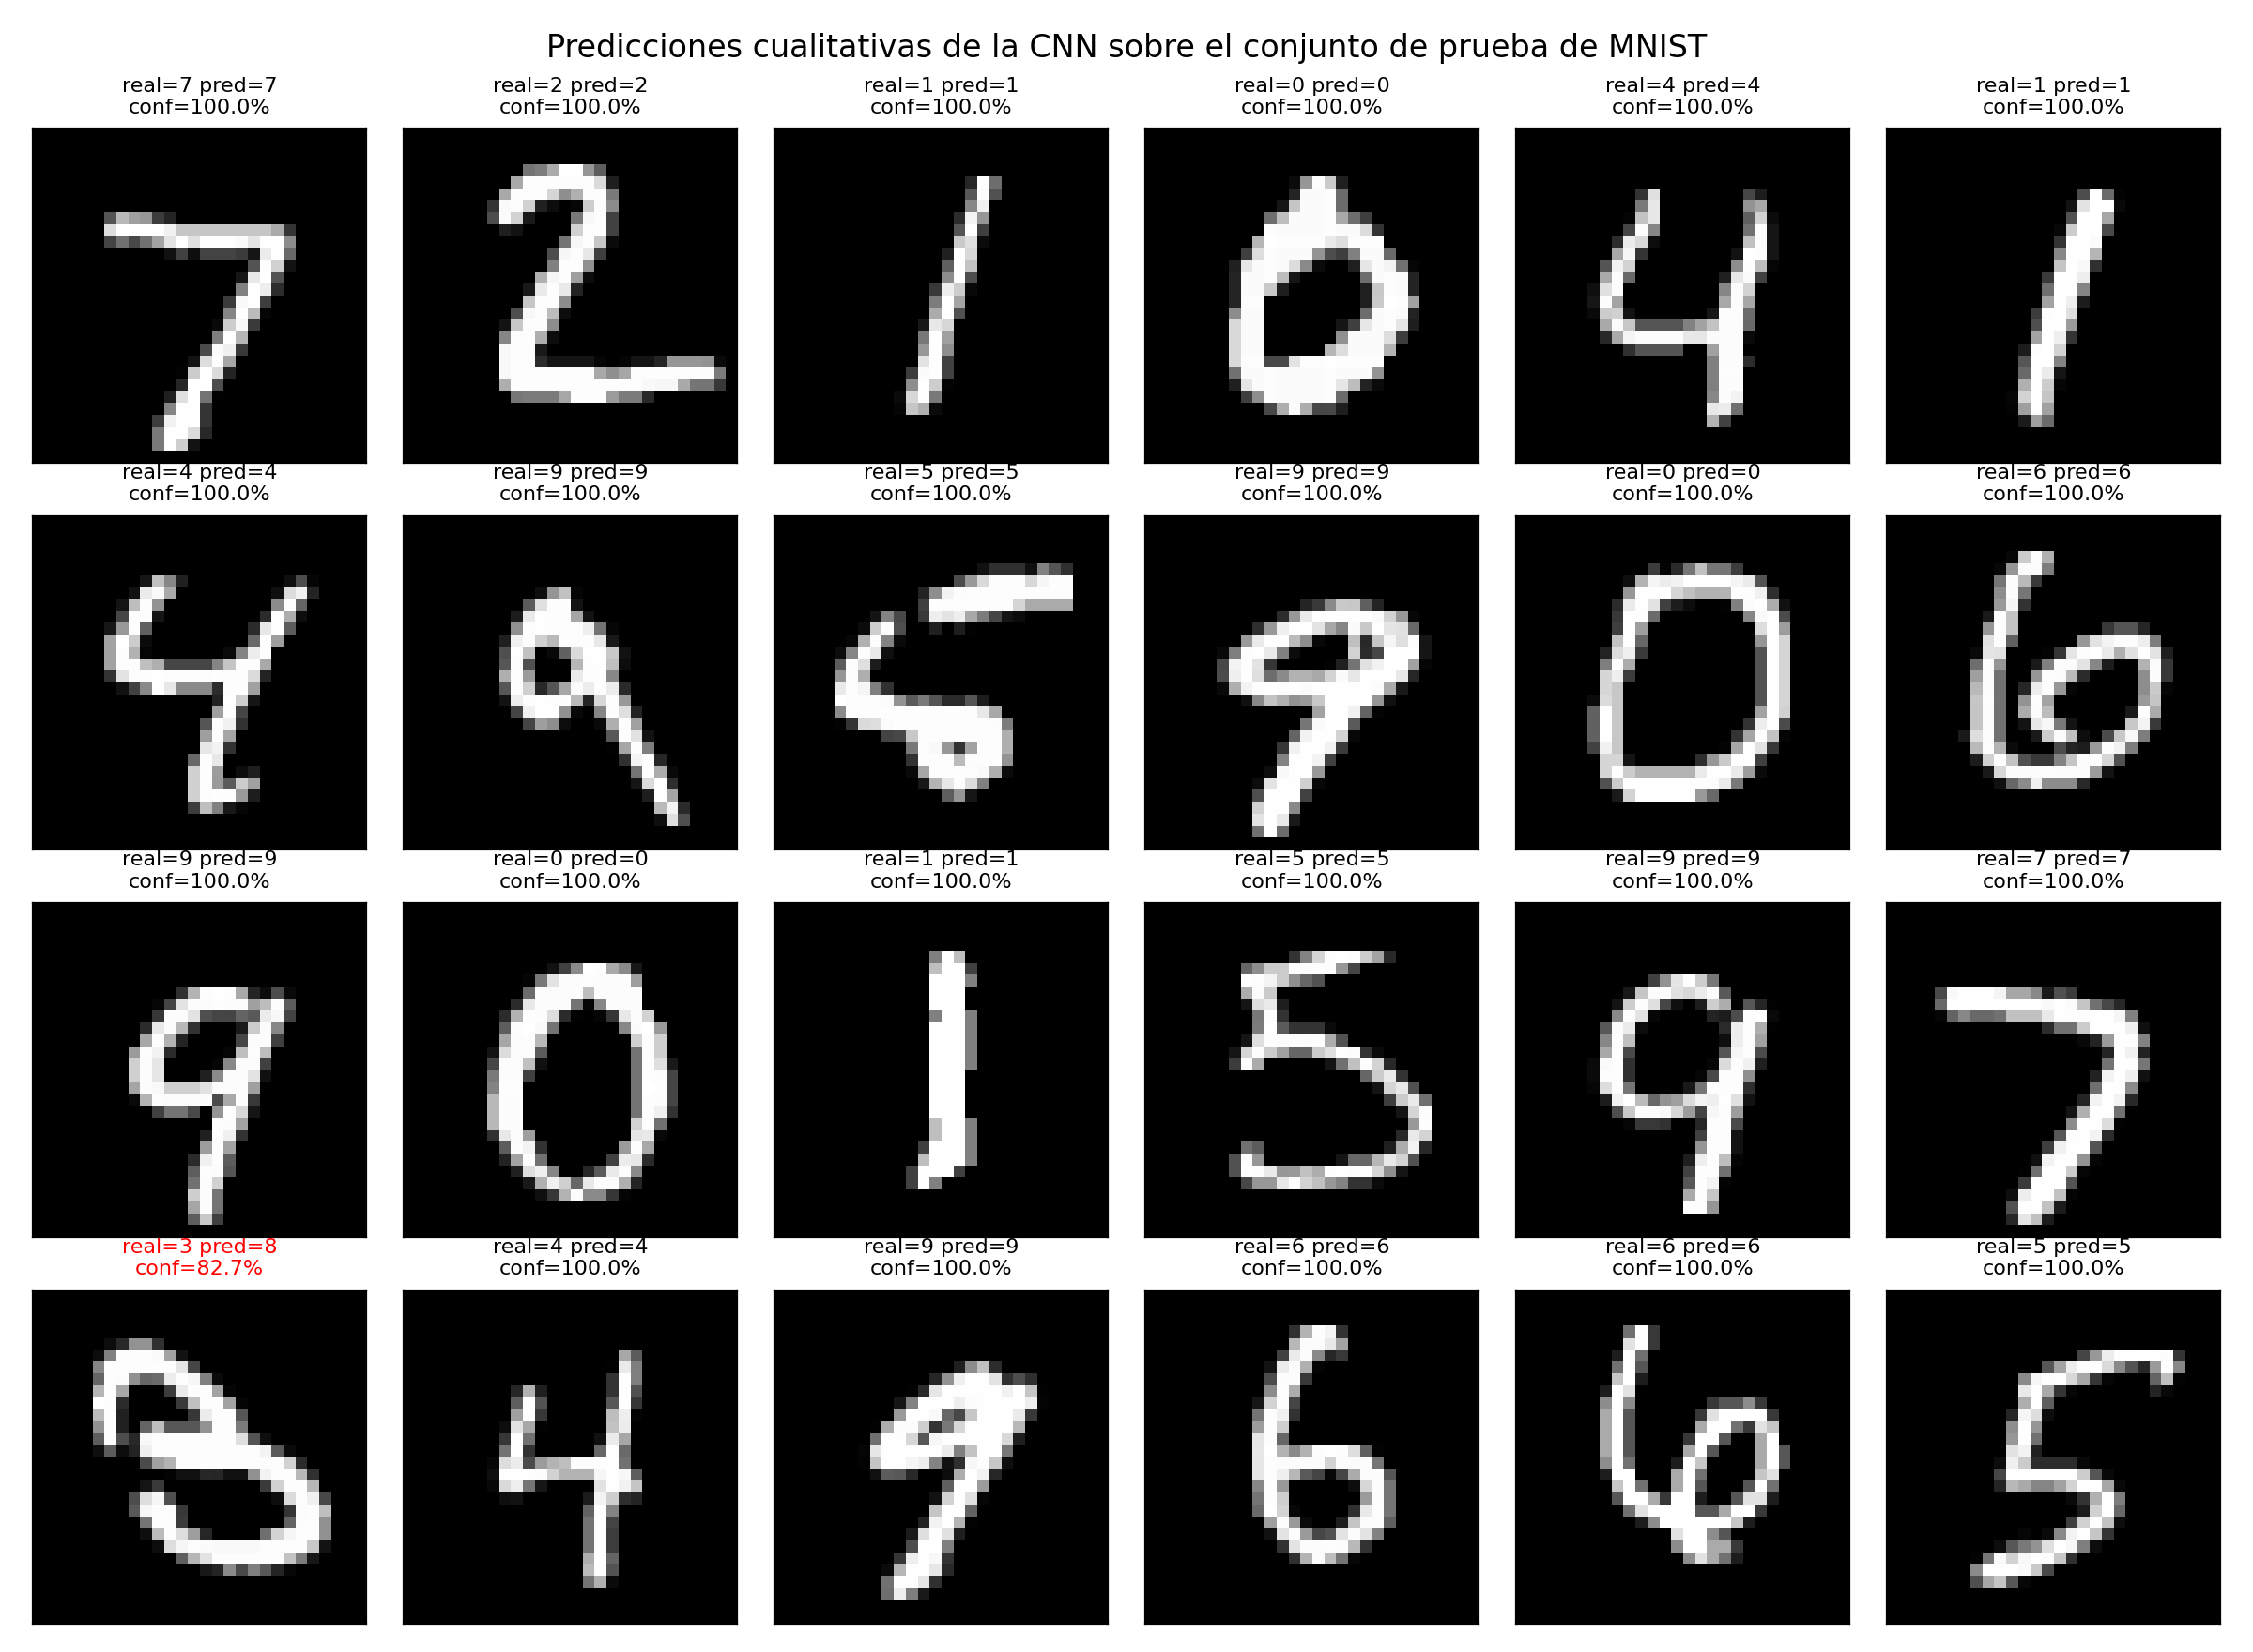
\includegraphics[width=3.5in]{cnn_predictions.png}
\caption{Ejemplos de predicciones de la CNN sobre imágenes de prueba de MNIST.}
\label{fig:predictions}
\end{figure}

De los 24 ejemplos, 23 fueron clasificados correctamente con una confianza softmax superior al 99.9\%. El único error de la muestra corresponde a un dígito 3 clasificado como 8 con una confianza de apenas 82.7\%, sensiblemente menor que la del resto de predicciones; este comportamiento es deseable, pues indica que el modelo asigna menor certeza precisamente al ejemplo que clasifica incorrectamente, en lugar de fallar con alta confianza.

\subsection{Discusión}
Los resultados confirman que, para una tarea de clasificación de imágenes de baja resolución y fondo uniforme como MNIST, el sesgo inductivo convolucional (localidad, compartición de pesos e invarianza aproximada a la traslación) se traduce en una convergencia más rápida —95.6\% de exactitud de prueba tras una sola época— y una exactitud final ligeramente superior a la reportada para un Vision Transformer de tamaño comparable entrenado bajo el mismo protocolo de optimización, tamaño de lote y número de pasos de \emph{warmup} \cite{dosovitskiy2020image}: 99.26\% frente a 98.68\%, con una pérdida de prueba menor (0.0260 frente a 0.0442). Esta diferencia es consistente con la literatura: los Transformers puros carecen de sesgo inductivo espacial y típicamente requieren mayor volumen de datos, aumentación o preentrenamiento para igualar a las CNN en régimen de datos moderados \cite{dosovitskiy2020image}, mientras que una CNN pequeña ya incorpora ese sesgo por construcción. Cabe notar que la CNN aquí implementada logra este resultado con aproximadamente un tercio menos de parámetros que el Transformer de referencia (206{,}922 frente a 305{,}034), lo que refuerza la eficiencia paramétrica de la convolución en este régimen.

% ==================
% # V. CONCLUSIÓN #
% ==================
\section{Conclusiones}

En este trabajo se implementó desde cero, en C++ y CUDA, una red neuronal convolucional compacta y se entrenó satisfactoriamente sobre el conjunto de datos MNIST, alcanzando una exactitud de prueba de 99.26\% (máxima de 99.28\%) tras 20 épocas de entrenamiento, con un consumo de memoria GPU de aproximadamente 1.17 GiB. Los resultados validan tanto la corrección de la implementación de bajo nivel de los componentes fundamentales de una CNN —convolución 2D vía \emph{im2col} y GEMM, \emph{max-pooling} con enrutamiento de gradiente por índice de máximo, activación ReLU, \emph{dropout} y el optimizador AdamW con programación de tasa de aprendizaje \emph{warmup} + coseno— como la eficacia del sesgo inductivo convolucional frente a una arquitectura puramente basada en atención de tamaño comparable entrenada bajo el mismo protocolo, para una tarea de clasificación de imágenes de baja complejidad.

Como trabajo futuro se plantea: (i) evaluar el modelo sobre conjuntos de datos de mayor complejidad (p. ej. CIFAR-10 o Fashion-MNIST), donde el sesgo inductivo convolucional podría ofrecer una ventaja aún mayor o, por el contrario, verse limitado por su alcance local; (ii) incorporar normalización por lotes (\emph{batch normalization}) y aumentación de datos (rotaciones, traslaciones, \emph{cutout}) para estudiar su efecto sobre la generalización; (iii) optimizar los kernels CUDA existentes, en particular la operación \emph{im2col}/\emph{col2im} y el GEMM tileado, mediante el uso de \emph{tensor cores} o de una jerarquía de \emph{tiling} más agresiva, con el fin de reducir el tiempo de entrenamiento por época; y (iv) extender la comparación cuantitativa con el Vision Transformer companion mediante métricas adicionales de calibración (p. ej. \emph{expected calibration error}) y de robustez frente a perturbaciones adversariales o de dominio.


% ==============
% # REFERENCIAS #
% ==============
\begin{thebibliography}{00}

\bibitem{lecun1998mnist}
Y. LeCun, L. Bottou, Y. Bengio, and P. Haffner, ``Gradient-based learning applied to document recognition,'' \emph{Proceedings of the IEEE}, vol. 86, no. 11, pp. 2278--2324, 1998.

\bibitem{krizhevsky2012imagenet}
A. Krizhevsky, I. Sutskever, and G. E. Hinton, ``ImageNet classification with deep convolutional neural networks,'' in \emph{Advances in Neural Information Processing Systems (NeurIPS)}, 2012, pp. 1097--1105.

\bibitem{dosovitskiy2020image}
A. Dosovitskiy, L. Beyer, A. Kolesnikov, D. Weissenborn, X. Zhai, T. Unterthiner, M. Dehghani, M. Minderer, G. Heigold, S. Gelly, J. Uszkoreit, and N. Houlsby, ``An image is worth 16x16 words: Transformers for image recognition at scale,'' in \emph{International Conference on Learning Representations (ICLR)}, 2021.

\bibitem{vaswani2017attention}
A. Vaswani, N. Shazeer, N. Parmar, J. Uszkoreit, L. Jones, A. N. Gomez, Ł. Kaiser, and I. Polosukhin, ``Attention is all you need,'' in \emph{Advances in Neural Information Processing Systems (NeurIPS)}, 2017, pp. 5998--6008.

\bibitem{nair2010rectified}
V. Nair and G. E. Hinton, ``Rectified linear units improve restricted Boltzmann machines,'' in \emph{Proceedings of the 27th International Conference on Machine Learning (ICML)}, 2010, pp. 807--814.

\bibitem{srivastava2014dropout}
N. Srivastava, G. Hinton, A. Krizhevsky, I. Sutskever, and R. Salakhutdinov, ``Dropout: A simple way to prevent neural networks from overfitting,'' \emph{Journal of Machine Learning Research}, vol. 15, no. 1, pp. 1929--1958, 2014.

\bibitem{he2015delving}
K. He, X. Zhang, S. Ren, and J. Sun, ``Delving deep into rectifiers: Surpassing human-level performance on ImageNet classification,'' in \emph{Proceedings of the IEEE International Conference on Computer Vision (ICCV)}, 2015, pp. 1026--1034.

\bibitem{loshchilov2017decoupled}
I. Loshchilov and F. Hutter, ``Decoupled weight decay regularization,'' in \emph{International Conference on Learning Representations (ICLR)}, 2019.

\end{thebibliography}

\end{document}
